\section{Chaos à Sichua}

\subsection*{Introduction}

Suite à la révélation de la connexion entre les différents troubles dans a ville et
la découverte de l'un des membres éminent du culte d'Azazel, le culte d'Azazel décide 
de répondre avec force. Ce chapitre de l'aventure commence par l'assassinat du 
principal allié des joueurs et par l'augmentation significative des troubles en ville.

\subsubsection*{Choisir sa voie}

Le groupe est introduit auprès du conseil des cinq. Ceux ci leur demande de 
résumer leurs découvertes. Les joueurs choisissent un patron parmis les cinq.

Selon le niveau de débrouillardise des joueurs, il faut les pousser plus ou moins.

Il y a trois voies possibles, l'infiltration de la guilde des voleurs, l'infiltration
démonistes (si ils n'ont pas été détruit), l'infiltration des chasseurs de monstres,
les troubles nécromantiques.

\subsection*{L'invasion de morts vivants}

\subsection*{Le Culte Démoniste}

\subsubsection*{Infiltration}
Si ils ne l'ont pas déjà, leur patron fournit l'amulette d'Azazel

\begin{figure}[htb!]
\center
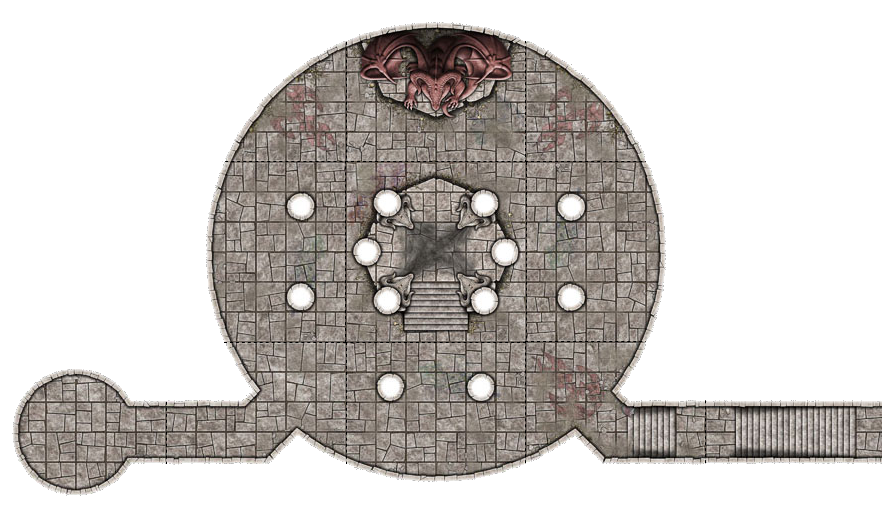
\includegraphics[width=7cm]{Maps/Temple.png}
\end{figure}

Le groupe se rend dans les quartiers où se trouvent le plus de démonistes. 
Alors qu'ils mènent leur enquête, ils sont guidé vers une auberge où se 
trouverait des cultistes. Alors que les joueurs sont dans l'auberge des sons 
étranges résonne dans le bâtiment. Le groupe est alors attaqué par un Vrock
(page \pageref{Vrock}). Lorsqu'ils trouvent le lieu d'origine de la bête, ils trouvent un 
pentacle de sang au sol et quelques cultistes qui se sont apparement saigné 
à mort pour l'invocation.

L'intérogatoire d'un survivant révèle que chaque meneur rassemble un petit 
cercle de fidèles et les dirigeants se regroupe dans une instance plus 
importante. Le groupe devra les infiltrer pour découvrir qui dirige réellement
le culte.

Dans le sous sol d'une auberge (potentielle aquisition du groupe)
Prendre la place d'un meneur -> combattre un Diable à chaines.
Meneur ancien tenancier "???"
Ses patrons "Godrik" "Keltar" "Ernoc"

Description de l'auberge, grande salle ronde au sous sol. A l'étage, les 
chambres sont surtout louée à des cultistes. Chambre principale occupée par le leader.

Participation a une première réunion.
Le groupe est demandeur d'exaction. Conundrum moral. Peuvent executer un comdamné à mort ou autre.
Proposition de duel (un contre un) en fin de réunion (challenge majeur). Les joueurs peuvent attendre une meilleure
occasion hors réunion (il faut ensuite convaincre le culte que la prise de 
pouvoir est légitime: autre combat) ou préparer la rencontre de fin de réunion avec des potions, buffs divers lors de la réunion suivante.


Appel auprès du grand chef. Réunion dans le cimetière du nord. Demande de rassembler des os d'humanoides 
pour une invocation. Ceux qui en ramèneront le plus participeront à l'invocation et gagneront les faveurs de Azazel.
Il sacrifie une jeune femme en fin de réunion sur l'autel.  Occasion en or de l'attrapé isolé.

Options: piller des catacombes ou s'attaquer à une tribu de gobelinoides en marge de la ville et trouver leur cimetière. Il faudra en ramener une carriole!

\subsubsection*{Piller les anciennes catacombes}

Les anciennes catacombes sont vieille de plusieurs siècles, peut être millénaires, elles datent d'une époque où 
les nécromanciens étaient trop nombreux et où il n'était pas raisonnable de conserver des corps 
en grande quantité dans la ville. Les catacombes se trovent à deux jours de marche environ au sud 
de Sichua, le voyage traverse des territoires vallonés et agricoles. Les catacombes se trouvent à
l'auré d'une grande forêt encore sauvage. Les rumeurs sont nombreuses et suffisament effrayante pour
avoir stoppé la progression de la civilisation dans cette direction. Si les joueurs mènent une enquête
dans les alentours sur ces rumeurs, un jet DC 12 en investigation leur permet de s'appercevoir qu'entre
les multiples histoires de fantômes, spèctres, goules et autre morts-vivants, il est aussi souvent 
question d'une sorcière faucheuse d'âmes.

Le patron des aventurier leur fournit une petit cariole avec sa mule et trois barils à remplir 
d'ossements. Un guide connaissant la région les accompagne aussi, malheureusement, celui-ci est
incapable de combattre efficacement (statistiques page \pageref{Eclaireur}). Lorsque le groupe
arrive sur place ils découvrent un ancien temple en grande partie détruit en l'honneur du dieu 
de la mort. Le temple est envahi par la végétation et la forêt alentour est particulièrement
épaisse et impénétrable, il semble impossible d'aller plus loin avec la carriole. Dans les 
décombres du temple derrière l'autel se trouve une arche de pierre avec des runes servant 
d'entrée à un tunnel, c'est très certainement l'entrée des catacombes. Un jet de religion
DC 15 permet d'interpreter ces runes magiques, celles-ci permettent de bloquer le passage
de tout mort-vivant dans un sens ou dans l'autre.

Affrontement de morts vivants qui semblent particulièrement excités.

Fantome en entrant

Arrivé aux catacombes les os semblent s'activer, 6 squeletes et minotaure.
Dans la salle une fouille rapide permet de trouver une lantern of revealing 
sur des ossements plus récents. Probablement ceux d'un pilleur de tombe, la 
lanterne parait intact ce qui attire l'oeil, l'objet semble magique.

Tombe sur une hag qui se considère propriétaire des ossements et compte bien tirer quelque chose des joueurs.
Pendant que ceux-ci visitent la crypte elle tue et remplace le guide des joueurs. Si les joueurs ne voient pas le coup
venir, elle hante l'un d'eux duran la nuit. Elle fera le nécessaire pour tuer un joueur et voler son âme avant de s'enfuir.

Au cas ou l'équipe arrive a tuer la hag, sur son corps ils trouvent plusieurs objets magiques, un 
anneau de barrière mentale (page \pageref{AnneauBarriereMentale})
et une flasque de fer (page \pageref{FlasqueFer}). Elle dispose aussi sur elle d'une statuette en
or, un jet religion DC 15 permet de connaitre une version primitive de Eril dieu de la justice.
Si les joueurs le ramène au temple de la justice, il l'échange contre le marteau de tonnerre.
Cette dernière si elle est activée 
révèle une jeune femme appeuré qui déclare
s'appeler Sélia et avoir été enlevé, c'était il y a fort longtemps et elle ne se souvient de rien
de sa vie passé. En fait c'est une succube, Joaline, (page \pageref{Succube}) qui 
tentera d'user de ses charmes sur l'un des joueurs
masculin de préférence. Si elle est découverte elle tentera de fuir. Elle porte un anneau de 
régeneration (page \pageref{AnneauRegeneration}).

Une fouille approfondie des catacombes durant une journée se fait sans rencontre supplémentaire
à l'exceptions de quelques squelettes (combats non joués). Un jet d'investigation DC 15 permet
de trouver un objet d'intérêt. Dans la tombe d'un barde se trouve une mandoline magique
(Canaith Mandolin, Instrument de Barde, pas sur AideDD. Faire un objet concient ou l'esprit d'un
ancien barde est piégé).

Passage niveau 6.

\subsubsection*{Chasse aux Gobelins}

Affrontement d'une troupe de chasseurs isolés

Combat pour leur ancien lieux de culte 

Poursuite pour échapper

\subsubsection*{Démanteler le culte démoniste}

Au retour en ville le groupe trouve une ville en émois et un combat éclate dès 
les faubourgs avec des diables: trois chiens des enfers 
(page \pageref{ChienEnfers}). Après ce combat, les joueurs apprennent
que la garde a du mal a maintenir la paix simplement dans les murs. Les faubourgs 
sont abandonnés aux diables. Lors de la prochaine réunion, il va falloir suivre
quelques leader cultistes et faire du ménage discrètement en attendant le gros 
évenement. 

En attendant l'appel les joueurs peuvent tenter de trouver l'un des cultes et tuer son 
leader. Ils peuvent ainsi s'attaquer à la ferme de la réunion qui est en fait le centre
d'un culte ou enqueter en ville. Quoiqu'il en soit, leur adversaire est un diable à 
chaine accompagné d'un chien des enfers (pages \pageref{DiableChaine} et \pageref{ChienEnfers}).

A la réunion suivante les cultistes se regroupent dans les faubourgs dans un petit champ
derrière une ferme. Le leader cultiste distribue des parchemins d'invocations de chiens 
des enfers et conseille à chacun d'invoquer massivement dans les jours qui viennent.
Le parchemin nécessite le sacrifice de trois personnes pour s'activer. En matière 
d'ossements, les membres du groupe gagnent la petite compétition. Le leader
les felicite de leur intelligence d'aller chercher l'exterieur de la ville. Il 
convoquera le guide du groupe lorsque tout sera pret pour l'invocation. (en cas d'échec
à la mission precedente, les joueurs doivent suivre le vaincoeur et prendre
sa place dans la plus grande discrétion).

Les membres du culte des joueurs demandent une invocation dans leur groupe, car il y
en a eu plusieurs pas loin. Certains membres quittent le groupe pour rejoindre
des voisins. Si les joueurs ne font pas quelque chose, ils reviennent pour les
abattres (trois Cult fanatics, un chien des enfers et un gladiateur 
(gants de force d'ogre) . Les joueurs 
peuvent s'attaquer aux voisins (meme troupe a vaincre), mais attention, il va falloir 
être discret et ne pas se griller dans le culte d'Azazel. Si l'invocation est 
effectuée par l'un des joueurs, sont prochain niveau est automatiquement un 
multiclassage sorcier (si il ne l'a pas déjà) avec Azazel comme patron. (Ce niveau 
pourra être annulé et repris comme un niveau du choix du joueur à la fin du chapitre).

L'appel vient finalement, rendez vous dans des caves sous les collines du sud.
Un véritable labyrinte où sont enmenés les ossements. Les joueurs sont attaqués
à la sortie de leur base par un concurrent mécontent d'avoir été doublé, c'est
un cambion, accompagné d'un chien des enfers (pages \pageref{Cambion} et \pageref{ChienEnfers}).
Ils peuvent les avoir tuer si ils ont suivi l'un des chefs cultistes lors de la 
réunion. Le cambion porte une armure d'écaille de mithril et 550 po. Nom: Aturik.
(Ajouter des trucs dans le hangar).

\subsection*{L'invocation}

Les joueurs sont convoqué dans une auberge du sud au pied des falaises 
sous la colline ou habite les familles fortunées. La cave de l'auberge s'étend 
sous la colline et les joueurs y trouvent un grand temple qui a été visiblement 
réamenaagé pour le culte d'Azazel. Seul le leader du culte est néanmoins invité à
l'interieur. Le temple est installée dans une grande caverne avec au fond une 
énorme statue d'Azazel. Au centre se trouve un pentacle géant où sont accumulés
tous les ossements rassemblés précédemment. Deux golems de chaire sont aussi
présent dans le temple avec Krassius Eldark qui indique à son invité que lui 
et les golems sont là pour sécurisé les lieux durant l'invocation. Si son rituel
devait être interrompu, le portail deviendrait instable et risquerait fortement 
de tout absorber!

Le rituel prend 1 minute (10 tours). Au premier tour apparaissent 3 quasit,
au deuxième tour deux shadow demons, au troisième tour un chasme et au cinquieme
tour un Vrock (page \pageref{Vrock}). Ces démons et diables attaquent les créatures
les plus proche d'eux de manière aléatoire. Les golems font écran pour protéger
Krassius. Au dixième tour un diable cornu nommé
Andear (page \pageref{DiableCornu}) apparait, celui ci idenifie immédiatement 
les aventuriers comme des traitres et agit de concert avec Krassius. Le seul moyen
de mettre fin au rituel avant qu'il soit complèter est de tuer Krassius. Celui-ci
n'agit pas durant les dix tours de l'invocation et reste concentré quoiqu'il arrive.
À la fin du rituel, ses pouvoirs magiques sont épuise et il se contente de s'éloigner
du portail puis d'utiliser ses cantrips dans le combat.

%TODO ajouter les démons et les liens correspondant.

Dans le cas où le rituel est annulé ou terminé, le portail se referme.
La fermeture du portail prend 3 tours causant des dégâts comme il suit. 
Durant ces trois tours les créatures à
moins de 6 mètres du pentacle doivent faire un jet de sauvegarde en force DC15, 
ils subissent 8d6 dommages de force et leur vitesse est divisée par deux jusqu'à 
la fin de leur prochain tour en cas d'échec ou subissent simplement la moitié des dégâts 
en cas de succès. Les objets non portés et les corps inanimés à porté du portail
sont aspirés et transportés dans les neufs enfers (localisation exact aléatoire).

Les personnages réstés à l'extérieur doivent passer quelques cultistes mineurs 
pour arriver au temple en toute discrétion. Il est important que les joueurs
indique quel trigger les fera intervenir ou entrer dans l'auberge pour éviter
une influence des évènements qu'ils ne sont pas sensé connaître. Un jet 
d'investigation DC 15 sur les alentours de l'auberge, leur permet de comprendre 
qu'il y a possiblement une partie troglodyte dans l'auberge.


En fin de combat, le maitre démoniste est identifié comme étant Krassius Eldark
le maitre des golems à la guilde des alchimistes. Il porte sur lui une baguette
de mage de guerre +2, amulette of proof against detection and location, bottes
elfiques.

Dans une petite alcove du temple, on peut trouver un bureau avec des documents 
interessant: des lettres d'échanges entre le culte et le maître de la guilde
des assassins
son clair. C'est cet assassin qui est son principal allié 
et le contact principal avec le maître "sur terre" depuis le départ de Soren  
"sous terre". Le dialogue est quelque peu cryptique et clairement cette invocation
interompu devait marqué une prise de pouvoir majeure pour le culte d'Azazel, mais
il reste un membre identifié en ville dont il faut se débarasser et il y a
un grand chef qui chapaute toute cette histoire, à moins que ce soit une référence 
à Azazel lui même. Difficile de comprendre.

Les documents indiquent aussi que cette nuit doit être assassiné le prévot des 
marchands, qui devrait facilement être remplacé par Krassius. Celui ci compte
mettre a disposition quelques golems pour patrouiller les rues durant la période
d'élection pour se garantir la victoire.
Enfin quelques objets interessant attirent l'attention des joueurs dans les tiroirs
du bureau: Alchemy Jug, Driftglobe et sending stones.

Lorsque les joueurs ressortent du temple, le groupe rencontre une troupe
en pleine chasse aux démons. Ceux-ci semblent imperturbables dans leur sport et 
se préoccupe plus de dénicher la plus grosse créature possible plutot que de
sauver les gens. Néanmoins les choses semblent sous contrôle car ils ont tué quelques
créatures déjà. A leur tête Magdan de Seryn, un cousin du duc, jeune général de l'armée
ducale.

A l'arrivé sur l'ilot, le groupe apprend que l'assassinat a malheureusement déjà eu 
lieu, mais dans les notes de Krassius, les avanturiers trouvent une liste
des localisations des chefs de culte locaux qui permetront aux autorités de les mettre
hors d'etat de nuire en quelques nuits.

Passage niveau 7


\subsection*{Le Club des Chasseurs}

Contact auprès de la guilde des alchimistes ou de la tour de magie


Identifie le maitre démoniste

\subsection*{L'infiltration de la guilde des voleurs}

Trouver un voleur pour être introduit auprès de la guilde

Quête catastrophique avec la halfeline Kirin pour dépouiller une client des dés d'argent.

-> Dead end les voleurs disparaissent les uns après les autres.


